% Name: Progress rings
% Description: Three rings that fill clockwise from the top to show how far each measure of a project has come, with the percentage in the middle.
% Tags: progress ring, radial progress, percentage, dashboard

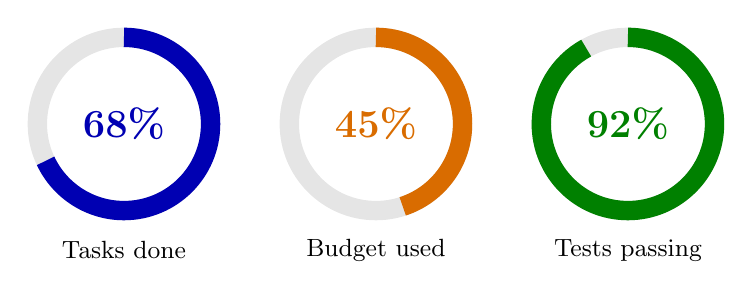
\begin{tikzpicture}[font=\small]
  \foreach \p/\name/\c [count=\i from 0] in {68/Tasks done/blue!70!black, 45/Budget used/orange!85!black, 92/Tests passing/green!50!black} {
    \begin{scope}[xshift=3.2*\i cm]
      \draw[gray!20, line width=7pt] (0,0) circle (1.1);
      \draw[\c, line width=7pt] (90:1.1) arc[start angle=90, end angle=90-3.6*\p, radius=1.1];
      \node[font=\Large\bfseries, text=\c] at (0,0) {\p\%};
      \node at (0,-1.6) {\name};
    \end{scope}
  }
\end{tikzpicture}
